\begin{auf}
    760
\end{auf}
Jemand befindet sich gleich weit von den beiden Lautsprechern einer Stereoanlage, die einen gegenseitigen Abstand von $d=4m$ haben, entfernt und hört einen reinen Ton. Er bewegt sich nun in seitliche Richtung um $x=0.5m$, bis der Ton wieder auf ein Lautstärkemaximum anschwillt.
\begin{enumerate}
    \item[a] Wie groß sind die Entfernungen $l_1$ und $l_2$ zu den Lautsprechern an diesem Ort?
    \item[b] Wie groß ist der Gangunterschied der eintreffenden	Schallwellen?
    \item[c] Welche Frequenz $f$ hat der Ton? Schallgeschwindigkeit	$340\frac{m}{s}$.
\end{enumerate}
\begin{figure}[h]
    \centering
    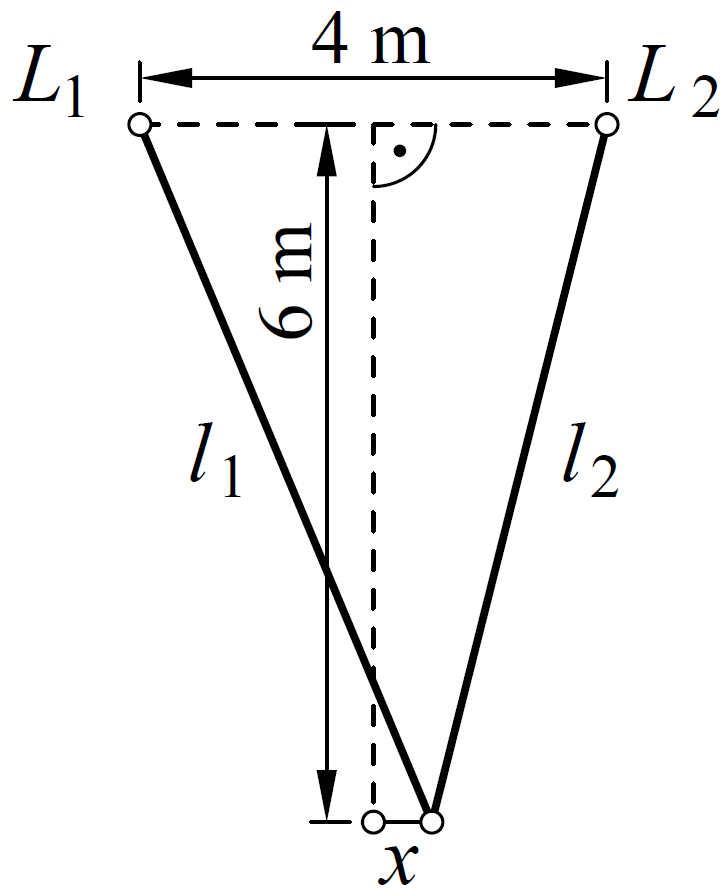
\includegraphics[height=5cm]{images/760_0.png}
    \caption{Versuchsaufbau Aufgabe 760}
\end{figure}